\documentclass[aspectratio=169]{beamer}
\usetheme{Madrid}
\usecolortheme{whale}
\definecolor{coforgenavy}{RGB}{13,40,79}
\definecolor{coforgeaccent}{RGB}{0,120,180}
\setbeamercolor{structure}{fg=coforgenavy}
\setbeamercolor{title}{fg=white,bg=coforgenavy}
\setbeamercolor{frametitle}{fg=white,bg=coforgenavy}
\setbeamercolor{block title}{fg=white,bg=coforgeaccent}
\setbeamerfont{frametitle}{series=\bfseries}
\setbeamertemplate{navigation symbols}{}
\setbeamertemplate{footline}{%
  \hbox{\begin{beamercolorbox}[wd=1\paperwidth,ht=2.5ex,dp=1.2ex,leftskip=1em,rightskip=1em]{structure}
  \footnotesize Team Qudit Creons --- TechCon Hackathon \hfill Use Case \#47 \hfill \insertframenumber/\inserttotalframenumber
  \end{beamercolorbox}}%
}
\usepackage[utf8]{inputenc}
\usepackage{tikz}
\usetikzlibrary{arrows.meta, positioning, shapes.geometric}

\title[Enterprise Mule Network Detection]{Enterprise AI Platform for Scam, Mule Network \& \\ Suspicious Transaction Detection}
\subtitle{Use Case \#47 --- TechCon Hackathon, Coforge}
\author{Team Qudit Creons \\[0.3em] \small Abhishek Raj \quad \textbar\quad Divyansh Singh}
\institute{Coforge --- \#CoforgeTechCon2026 \quad \#CoforgeHackathon}
\date{Idea Submission --- 7 August 2026}

\begin{document}

\begin{frame}
\titlepage
\end{frame}

% ---------------------------------------------------------
\begin{frame}{Domain \& Vision}
\textbf{Domain:} Banking, Financial Services \& Insurance (BFSI) \\
\textbf{Sub-domain:} Fraud Operations \& Anti-Money Laundering (AML)

\vspace{1em}
\begin{block}{Vision Statement}
Deliver an enterprise-grade, explainable, real-time platform that gives fraud investigators a unified view of mule networks and scam patterns --- so suspicious money movement is stopped \emph{before cash-out}, not reconstructed after the loss, at the scale and reliability an enterprise fraud desk demands.
\end{block}

\vspace{1em}
\textbf{Why it matters:} At enterprise scale --- millions of transactions across business units daily --- fraud losses are driven not by single bad transactions but by \emph{networks} of mule accounts moving funds in coordinated patterns. Row-level rule engines miss these patterns, and human reviewers cannot trace them manually at volume.
\end{frame}

% ---------------------------------------------------------
\begin{frame}{Problem Statement}
Current fraud operations rely on static, transaction-level rules that:
\begin{itemize}
\item Evaluate each transaction in isolation, missing coordinated multi-account patterns
\item Generate high false-positive volumes, overwhelming investigator capacity
\item Produce alerts with no explainable evidence trail, slowing case resolution
\item Detect fraud \emph{after} funds have already moved through the network
\end{itemize}

\vspace{0.5em}
\begin{block}{Core gap}
No unified system connects account-level relationships (the graph) with transaction-level anomaly signals (the data) to catch mule networks \emph{while} they are active.
\end{block}
\end{frame}

% ---------------------------------------------------------
\begin{frame}{Use Cases (1-liners)}
\begin{enumerate}
\item \textbf{Fan-out smurfing} --- one compromised account rapidly splits funds across many mule accounts
\item \textbf{Fan-in aggregation} --- many small transfers converge into one mule account, which cashes out fast
\item \textbf{Layering chains} --- funds bounce through a sequence of accounts to obscure origin
\item \textbf{Rapid pass-through} --- a mule account receives a large deposit and forwards it within minutes
\item \textbf{Real-time risk scoring} --- every transaction/account scored and routed to investigators only above threshold
\end{enumerate}
\end{frame}

% ---------------------------------------------------------
\begin{frame}{MVP Scope --- What We Build in the Hackathon}
\begin{columns}[T]
\begin{column}{0.5\textwidth}
\textbf{In scope}
\begin{itemize}
\small
\item Synthetic account/transaction dataset (no company data provided)
\item Account-transaction graph construction
\item Hybrid rule + ML detection for the 4 mule patterns
\item Real-time risk scoring API
\item Investigator dashboard: network graph + case explanation
\end{itemize}
\end{column}
\begin{column}{0.5\textwidth}
\textbf{Out of scope}
\begin{itemize}
\small
\item Live core-banking integration
\item Regulatory filing / SAR automation
\item Multi-currency, cross-border compliance rules
\item Production-grade auth \& security hardening
\end{itemize}
\end{column}
\end{columns}

\vspace{0.5em}
\footnotesize \textbf{Post-hackathon enterprise roadmap:} core-banking connectors, regulatory reporting, multi-tenant deployment, and hardened security are deliberately deferred --- the MVP is architected so each plugs in without a redesign.
\end{frame}

% ---------------------------------------------------------
\begin{frame}{Solution Approach --- Architecture}
\centering
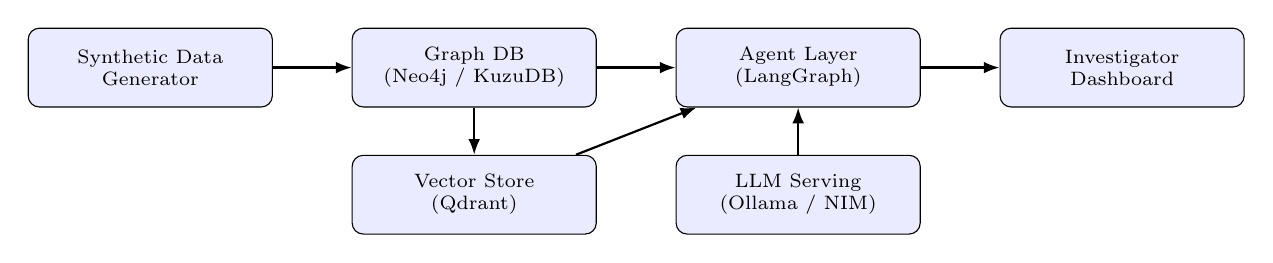
\begin{tikzpicture}[
  node distance=0.6cm and 1cm,
  box/.style={draw, rounded corners, minimum width=3.1cm, minimum height=1cm, align=center, font=\scriptsize, fill=blue!8},
  arr/.style={-{Latex[length=2mm]}, thick}
]
\node[box] (data) {Synthetic Data\\Generator};
\node[box, right=of data] (graph) {Graph DB\\(Neo4j / KuzuDB)};
\node[box, right=of graph] (agents) {Agent Layer\\(LangGraph)};
\node[box, right=of agents] (dash) {Investigator\\Dashboard};

\node[box, below=of graph] (vec) {Vector Store\\(Qdrant)};
\node[box, below=of agents] (llm) {LLM Serving\\(Ollama / NIM)};

\draw[arr] (data) -- (graph);
\draw[arr] (graph) -- (agents);
\draw[arr] (agents) -- (dash);
\draw[arr] (vec) -- (agents);
\draw[arr] (llm) -- (agents);
\draw[arr] (graph.south) -- (vec.north);
\end{tikzpicture}

\vspace{0.5em}
\footnotesize Detection agent (graph pattern + anomaly scoring) $\rightarrow$ Explanation agent (LLM narrates evidence) $\rightarrow$ Dashboard surfaces ranked, explainable cases.

\vspace{0.3em}
\footnotesize \textbf{Enterprise design principles:} stateless agent workers (horizontal scale-out), graph queries isolated from transactional writes, every scored decision logged for audit trail.
\end{frame}

% ---------------------------------------------------------
\begin{frame}{Solution Approach --- Open-Source Stack}
\small
\begin{tabular}{ll}
\textbf{Layer} & \textbf{Tool} \\
\hline
Graph relationships & Neo4j Community / KuzuDB \\
Vector retrieval & Qdrant \\
Hybrid graph+vector RAG & LlamaIndex PropertyGraphIndex \\
Agent orchestration & LangGraph \\
LLM serving (local) & Ollama --- Llama 3.3 70B / Qwen2.5-Coder \\
LLM serving (cloud fallback) & NVIDIA NIM (Nemotron, free credits) \\
App / session state & SQLite \\
\end{tabular}

\vspace{1em}
\begin{block}{Why this stack}
Every layer maps directly to the suggested open-source AI stack --- no proprietary dependency, runs on a free-tier cloud instance, and the graph+vector hybrid is what the use case's own detection logic requires (relationship patterns, not just row anomalies). All components are open-source and self-hostable, avoiding vendor lock-in for an enterprise rollout beyond the hackathon.
\end{block}
\end{frame}

\end{document}
